\chapter{Methodik}
\label{chap:methodik}

Für die Segmentierung der Marsoberfläche wird der Ansatz von Kanezaki \etal \cite{kanezaki_18} aus Unterabschnit~\ref{ssec:kanezaki} abgewandelt. Das Ziel besteht daraus, eine Eingabebilddatei durch neuronale Netze zu segmentieren, allerdings ohne vorhandene Ground Truth.

Zur Modifikation des genannten Algorithmus existieren viele unterschiedliche Möglichkeiten, einzelne Elemente zu ersetzen, welche in den folgenden Abschnitten beschrieben werden.

\section{Initialisierung}
\label{sec:initialisierung}

Die wohl wichtigste Veränderung des ursprünglichen Algorithmus besteht aus der Modifizierung des Initialisierungsalgorithmus.

Der von Kanezaki \etal genutzte SLIC-Algorithmus eignet sich zwar gut für die meisten mehrfarbigen Fotografien, da die Aufnahmen der Marsoberfläche allerdings nur in Graustufen vorhanden sind, würden so hier keine guten Ergebnisse produziert werden.

\begin{figure}[h!]
	\centering
	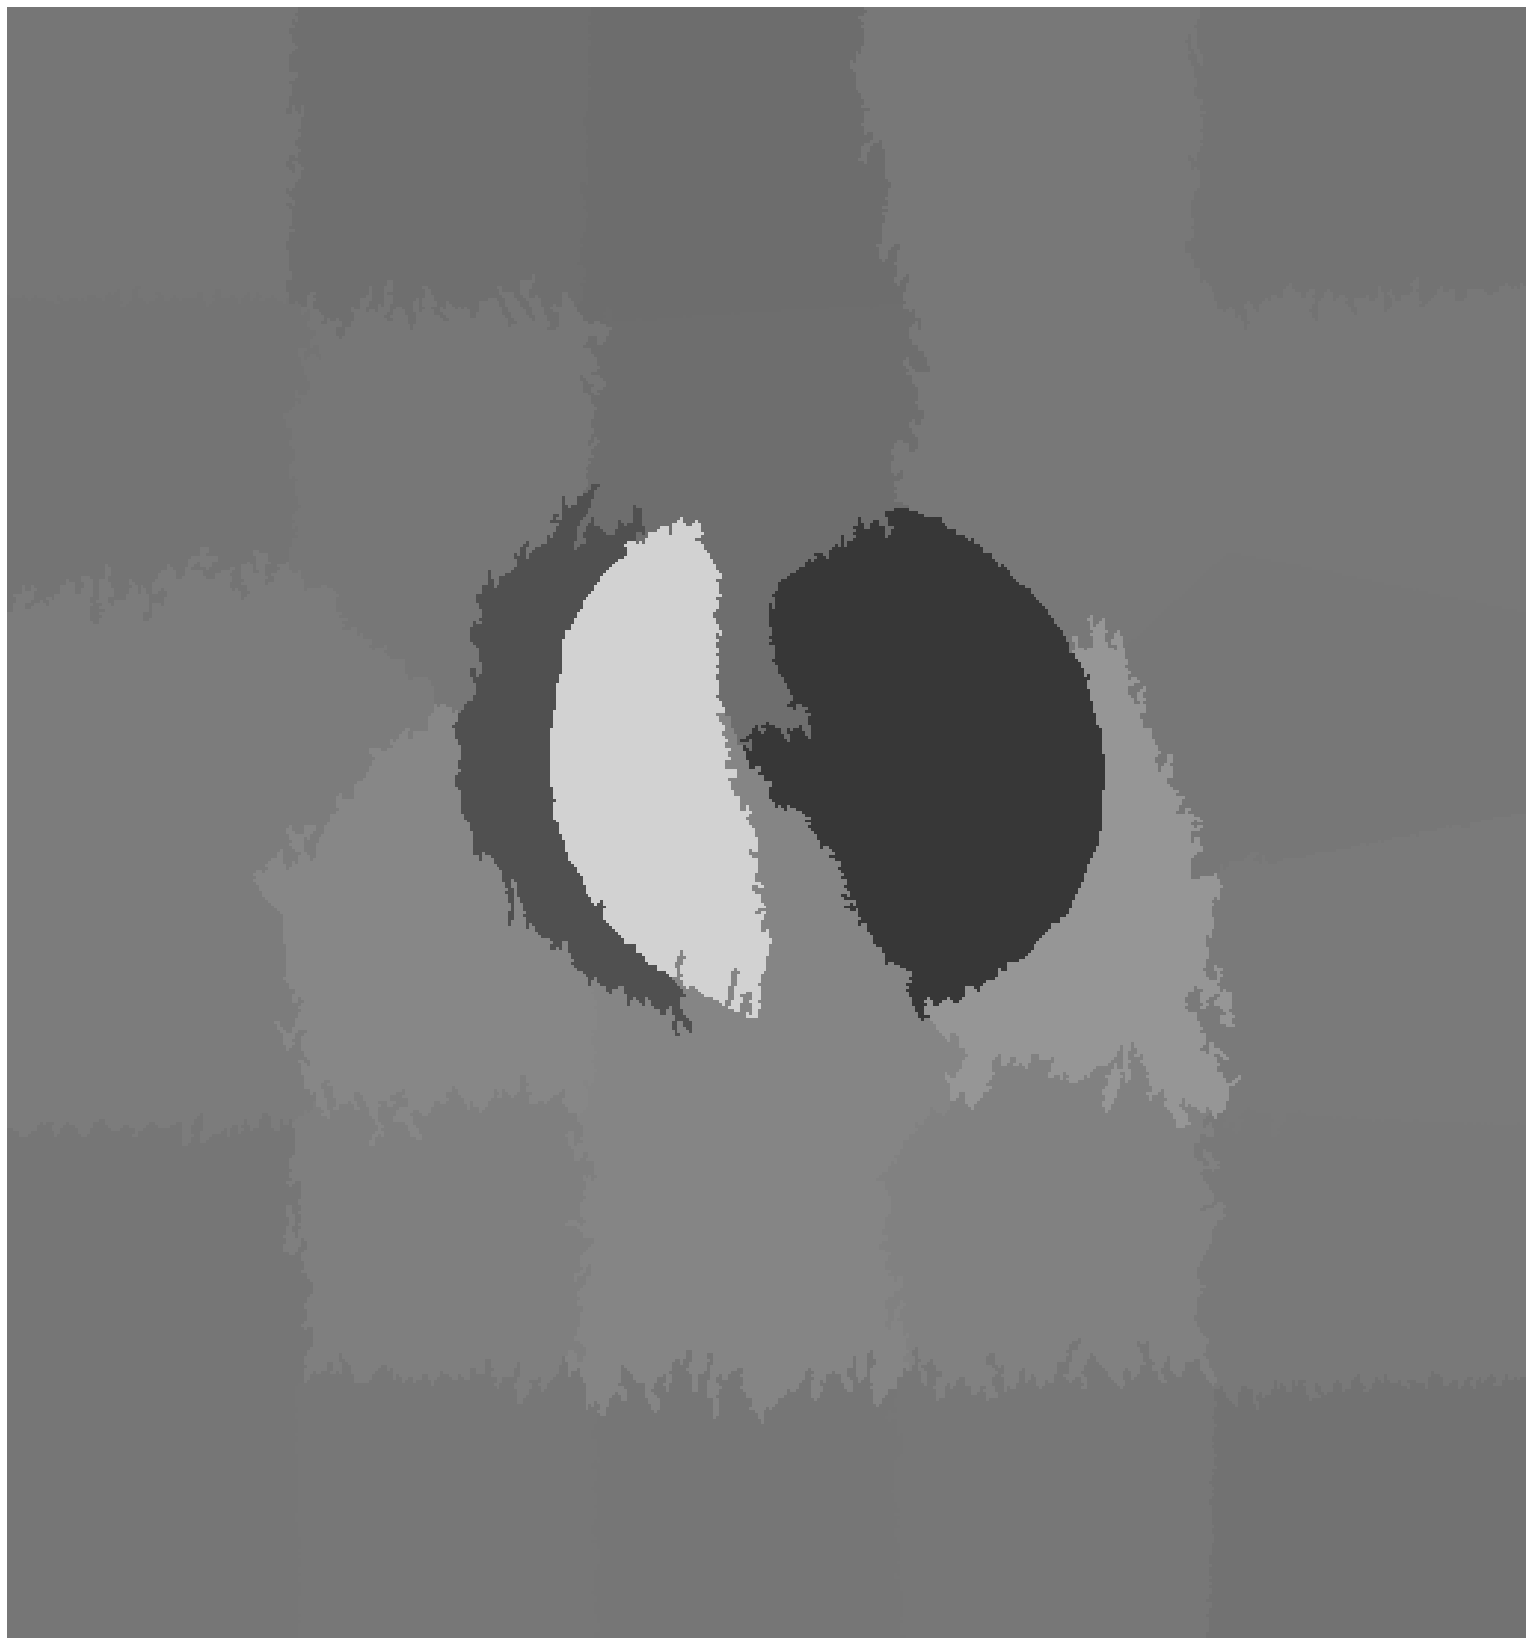
\includegraphics[width=0.35\textwidth,keepaspectratio]{images/gen/GEN_slic_crater.png}
	\captionsetup{format=plain,width=0.35\textwidth}
	\caption{Ergebnis des SLIC-Algorithmus angewandt auf eine Graustufenaufnahme eines Kraters}
	\label{fig:slic_crater}
\end{figure}

So ergibt ein Clustering des Kraters aus \figurename~\ref{fig:ex_crater} durch den SLIC-Algorithmus \cite{achanta_10} das in \figurename~\ref{fig:slic_crater} sichtbare Ergebnis.\footnote{SLIC-Implementierung: \textit{scikit-image}\\Parameter: \textit{compactness}=20, \textit{n\_segments}=30\\Cluster gefüllt mit ihren jeweiligen Durchnittshelligkeitswerten} Dort ist erkennbar, dass der Krater in jeweilige Licht- und Schattenregionen (bedingt durch den Lichteinfall im flachen Winkel) unterteilt wird. Dieses Phänomen wird sich zwar in \ref{sec:craterdetection} zu nutze gemacht, ist hier allerdings ungewollt.

Wenn nun der in Unterabschnitt~\ref{ssec:kanezaki} beschriebene Ansatz verfolgt wird, wird das neuronale Netz daraufhin trainiert, eine Aufnahme anhand ihrer Helligkeitsinformationen hin zu trainieren. Da dies nicht gewollt ist, wird statt einem farb-/helligkeitsbasierten Clusteringalgorithmus wie SLIC ein texturbasiertes Clustering genutzt.

\subsection{Gewichtungen}

\section{Netzwerkarchitektur}

\section{Abbruchkriterium}

\section{Anpassungen für mehrfarbige Fotografien}